\section{Experiment}
\subsection{Experiment Settings}

\noindent \textbf{Implementation Details.}
We evaluate the effectiveness of our method on two representative dLLMs, including LLaDA-8B-Instruct~\citep{nie2025large} and Dream-7B-Instruct~\citep{ye2025dream}.
For long-context evaluation, we follow the strategy of LongLLaDA~\citep{liu2025longllada} to ensure reliable performance on extended sequences.
All experiments were conducted on 8 × NVIDIA A100 80GB GPUs. Additional details are provided in Appendix~\ref{implement details}.

\subsection{Main Results}
\begin{table*}[t!]
    \centering
    \small
    \caption{LongBench results for LLaDA-8B and Dream-7B with specific KV cache budgets (B=32 and B=128). Best result in each column within a budget section is in \textbf{bold}.}
    \label{tab:main_b32_b128_results}
    \setlength{\tabcolsep}{3pt} 
    \renewcommand{\arraystretch}{1.1}
    \resizebox{\textwidth}{!}{%
    \begin{tabular}{@{}l*{15}{c}@{}}
        \toprule
        \textbf{Method} & \multicolumn{2}{c}{Single-Doc. QA} & \multicolumn{3}{c}{Multi-Doc. QA} & \multicolumn{3}{c}{Summarization} & \multicolumn{3}{c}{Few-shot Learning} & \multicolumn{1}{c}{Synthetic} & \multicolumn{2}{c}{Code} & \makecell{Ave. \\ Score} \\
        
        \cmidrule(lr){2-3} \cmidrule(lr){4-6} \cmidrule(lr){7-9} \cmidrule(lr){10-12} \cmidrule(lr){13-13} \cmidrule(lr){14-15}

        & \rotatebox[origin=c]{-45}{Qasper} & \rotatebox[origin=c]{-45}{MF-en} & \rotatebox[origin=c]{-45}{HotpotQA} 
        & \rotatebox[origin=c]{-45}{2WikiMQA} & \rotatebox[origin=c]{-45}{Musique} 
        & \rotatebox[origin=c]{-45}{GovReport} & \rotatebox[origin=c]{-45}{QMSum} & \rotatebox[origin=c]{-45}{MultiNews}
        & \rotatebox[origin=c]{-45}{TREC} & \rotatebox[origin=c]{-45}{TriviaQA} & \rotatebox[origin=c]{-45}{SAMSum}
        & \rotatebox[origin=c]{-45}{PRe}
        & \rotatebox[origin=c]{-45}{Lcc} & \rotatebox[origin=c]{-45}{RB-P}
        & \\
        
        \midrule
        \multicolumn{16}{c}{\large \textbf{LLaDA-8B-Instruct}} \\
        \midrule
        \multicolumn{16}{c}{\small Full KV Cache} \\
        \midrule
    \textcolor{gray}{dLLM w/o Cache} & \textcolor{gray}{16.96} & \textcolor{gray}{31.31} & \textcolor{gray}{14.68} & \textcolor{gray}{17.60} & \textcolor{gray}{11.48} & \textcolor{gray}{29.24} & \textcolor{gray}{21.93} & \textcolor{gray}{27.58} & \textcolor{gray}{65.20} & \textcolor{gray}{47.98} & \textcolor{gray}{40.51} & \textcolor{gray}{98.17} & \textcolor{gray}{65.69} & \textcolor{gray}{59.57} & \textcolor{gray}{39.14} \\
    \textcolor{gray}{dLLM w/ Cache} & \textcolor{gray}{15.26} & \textcolor{gray}{29.62} & \textcolor{gray}{13.87} & \textcolor{gray}{17.17} & \textcolor{gray}{10.44} & \textcolor{gray}{29.75} & \textcolor{gray}{22.06} & \textcolor{gray}{26.68} & \textcolor{gray}{66.00} & \textcolor{gray}{44.94} & \textcolor{gray}{41.86} & \textcolor{gray}{97.44} & \textcolor{gray}{66.07} & \textcolor{gray}{59.34} & \textcolor{gray}{38.61} \\

        \midrule
        \multicolumn{16}{c}{\small B=32} \\
        \midrule
        SnapKV & 9.10 & 17.49 & \textbf{17.38} & 16.45 & 8.06 & \textbf{9.92} & 12.21 & 13.95 & 39.25 & 54.32 & 16.41 & 55.00 & 39.90 & 29.08 & 24.18 \\
        PyramidKV & 9.90 & 12.12 & 14.46 & 14.62 & 8.18 & 9.10 & 8.83 & 12.36 & 26.42 & 53.26 & 14.51 & 28.00 & 39.18 & 27.66 & 19.90 \\
        SqueezeAttention & 11.49 & 14.72 & 16.66 & 15.42 & 8.15 & 9.28 & 10.49 & 14.86 & 43.50 & 53.67 & 15.73 & 52.00 & 33.60 & 25.56 & 23.22 \\
        AdaKV & 11.15 & 16.21 & 16.69 & \textbf{16.98} & 7.48 & 9.10 & 10.44 & 14.23 & 39.17 & \textbf{55.69} & 19.00 & 59.50 & 37.21 & 26.40 & 24.23 \\
        \rowcolor{lightgreen} \textbf{MaskKV (Ours)} & \textbf{14.61} & \textbf{24.45} & 17.05 & 15.68 & \textbf{12.50} & 9.54 & \textbf{14.33} & \textbf{16.43} & \textbf{40.42} & 54.64 & \textbf{29.28} & \textbf{90.33} & \textbf{56.08} & \textbf{42.21} & \textbf{31.25} \\
        \midrule
        \multicolumn{16}{c}{\small B=128} \\
        \midrule
        SnapKV & 17.42 & 26.65 & 15.88 & 17.44 & 7.99 & 11.50 & 11.69 & 18.89 & 50.83 & 55.60 & 20.72 & 80.00 & 54.90 & 39.33 & 30.63 \\
        PyramidKV & 15.71 & 25.20 & 16.22 & 16.20 & 8.47 & 10.09 & 11.06 & 17.22 & 39.92 & 55.03 & 23.49 & 83.25 & 54.00 & 40.50 & 29.74 \\
        SqueezeAttention & 14.46 & 17.64 & \textbf{18.12} & \textbf{17.97} & 8.00 & 13.46 & 10.69 & 19.46 & 52.67 & 54.71 & 17.04 & 71.00 & 48.30 & 32.51 & 28.29 \\
        AdaKV & 19.42 & 24.68 & 17.06 & 17.57 & 8.82 & 11.85 & 9.51 & 18.49 & 49.92 & \textbf{57.90} & 21.03 & 78.00 & 54.64 & 36.27 & 30.37 \\
        \rowcolor{lightgreen} \textbf{MaskKV (Ours)} & \textbf{20.21} & \textbf{29.84} & 15.78 & 16.65 & \textbf{11.83} & \textbf{13.60} & \textbf{17.67} & \textbf{20.78} & \textbf{57.00} & 46.06 & \textbf{37.28} & \textbf{98.17} & \textbf{61.61} & \textbf{51.86} & \textbf{35.60} \\
        \midrule
        \multicolumn{16}{c}{\large \textbf{Dream-v0-Instruct-7B}} \\
        \midrule
        \multicolumn{16}{c}{\small Full KV Cache} \\
        \midrule
\textcolor{gray}{dLLM w/o Cache} & \textcolor{gray}{28.17} & \textcolor{gray}{36.23} & \textcolor{gray}{27.65} & \textcolor{gray}{32.43} & \textcolor{gray}{11.83} & \textcolor{gray}{5.04} & \textcolor{gray}{14.29} & \textcolor{gray}{5.95} & \textcolor{gray}{73.00} & \textcolor{gray}{89.25} & \textcolor{gray}{37.84} & \textcolor{gray}{16.92} & \textcolor{gray}{38.91} & \textcolor{gray}{45.08} & \textcolor{gray}{33.04} \\
\textcolor{gray}{dLLM w/ Cache} & \textcolor{gray}{26.55} & \textcolor{gray}{39.86} & \textcolor{gray}{27.66} & \textcolor{gray}{32.09} & \textcolor{gray}{11.12} & \textcolor{gray}{4.40} & \textcolor{gray}{13.89} & \textcolor{gray}{5.51} & \textcolor{gray}{73.50} & \textcolor{gray}{89.59} & \textcolor{gray}{36.07} & \textcolor{gray}{12.05} & \textcolor{gray}{39.88} & \textcolor{gray}{45.57} & \textcolor{gray}{32.70} \\

        \midrule
        \multicolumn{16}{c}{\small B=32} \\
        \midrule
        SnapKV & 17.75 & 26.82 & 22.39 & \textbf{27.91} & 7.53 & \textbf{2.65} & \textbf{12.58} & 1.95 & 28.25 & 66.14 & 23.67 & 17.50 & 22.75 & 23.87 & 21.55 \\
        PyramidKV & 14.55 & 24.51 & 22.41 & 15.27 & 6.90 & 2.62 & 11.89 & 2.15 & 28.00 & 57.55 & 24.17 & 11.50 & 22.02 & 22.22 & 18.98 \\
        SqueezeAttention & 17.62 & 30.44 & 20.07 & 26.15 & 7.42 & 2.62 & 11.83 & 2.19 & 26.25 & 72.17 & 24.52 & 17.00 & 20.91 & 23.41 & 22.00 \\
        AdaKV & 17.09 & 25.42 & 23.64 & 24.77 & 7.55 & 2.58 & 12.46 & 1.89 & 27.75 & 69.77 & 25.21 & 18.83 & 21.67 & 24.98 & 21.69 \\
        \rowcolor{lightgreen} \textbf{MaskKV (Ours)} & \textbf{18.53} & \textbf{33.76} & \textbf{32.92} & 24.53 & \textbf{11.02} & 2.59 & 11.98 & \textbf{2.25} & \textbf{33.25} & \textbf{86.47} & \textbf{27.55} & \textbf{20.00} & \textbf{24.89} & \textbf{27.40} & \textbf{25.51} \\
        \midrule
        \multicolumn{16}{c}{\small B=128} \\
        \midrule
        SnapKV & \textbf{22.36} & 39.02 & 30.28 & 32.27 & 11.51 & 2.72 & \textbf{13.20} & 2.72 & 38.00 & 87.17 & 28.69 & \textbf{26.05} & \textbf{32.55} & 36.51 & 28.79 \\
        PyramidKV & 17.31 & 36.59 & 25.21 & 24.38 & 10.99 & 2.77 & 12.75 & 2.90 & 39.75 & 84.83 & 29.71 & 24.00 & 30.26 & 30.33 & 26.56 \\
        SqueezeAttention & 19.36 & 36.19 & 28.35 & 29.79 & 10.25 & 2.81 & 13.11 & 2.64 & 33.00 & 85.99 & 29.25 & 25.00 & 27.11 & 31.92 & 26.77 \\
        AdaKV & 21.97 & \textbf{39.68} & 33.24 & 31.57 & 11.38 & 2.69 & 13.15 & 2.80 & 38.75 & 88.51 & 30.43 & 24.25 & 31.46 & \textbf{37.28} & 29.08 \\
        \rowcolor{lightgreen} \textbf{MaskKV (Ours)} & 21.49 & 39.23 & \textbf{38.25} & \textbf{33.99} & \textbf{14.76} & \textbf{2.86} & 12.48 & \textbf{3.19} & \textbf{53.50} & \textbf{88.69} & \textbf{30.97} & 21.92 & 30.71 & 34.79 & \textbf{30.49} \\
        \bottomrule
    \end{tabular}
    } 
\end{table*}
\noindent \textbf{Preserving Accuracy with Reduced Cache.}
As shown in Tab.~\ref{tab:main_b32_b128_results}, our method consistently surpasses prior cache-eviction strategies on specific budgets. Under the extreme 32 KV budget, it outperforms the best competing baseline by 7.02 points on LLaDA-8B. Notably, our method can even surpass the full-context dLLM-Cache baseline, likely because eviction removes distracting noise from the context and enhances the model's focus.

\noindent \textbf{Stable Performance across Varied Budgets.}
As shown in Fig.\ref{fig:across_size}, with a 256~KV budget, our method retains 94.33\% of the dLLM‑Cache baseline's performance on \textbf{LLaDA} and 98.66\% on \textbf{Dream}, achieving the best results. This advantage holds across all KV budgets and remains strong even in extremely low‑budget regimes where autoregressive models typically collapse~\citep{xiao2023efficient}. We attribute this robustness to bidirectional attention, which integrates information from the entire sequence to form richer KV representations, enabling aggressive pruning with preserving high generation quality.

\begin{figure}[t]
  \centering
  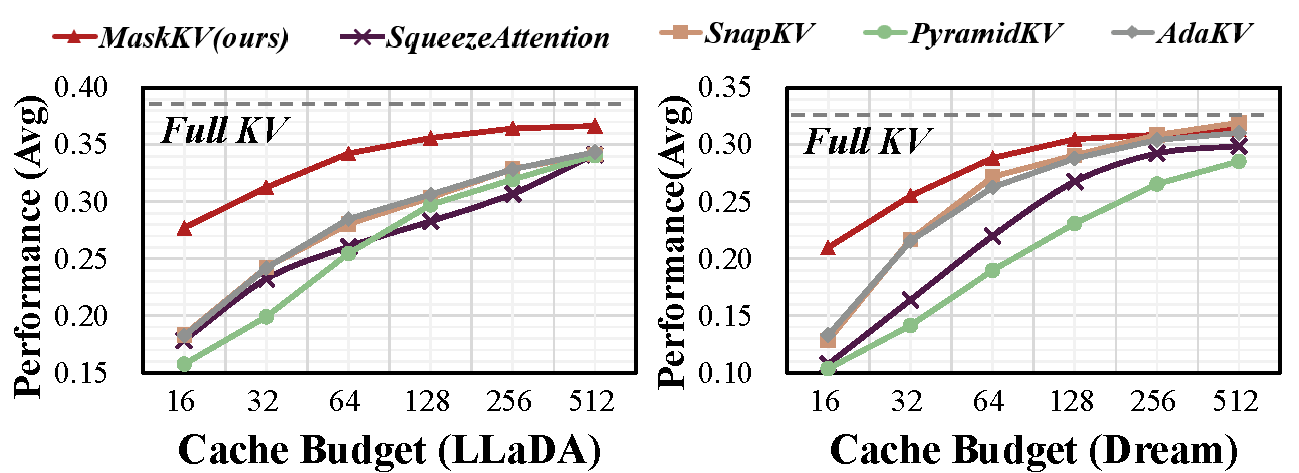
\includegraphics[width=\columnwidth]{figure/across_budget_new.pdf}
  \caption{Average LongBench performance across varying KV cache sizes.}
  \label{fig:across_size}
\end{figure}
\begin{figure}[t]
  \centering
  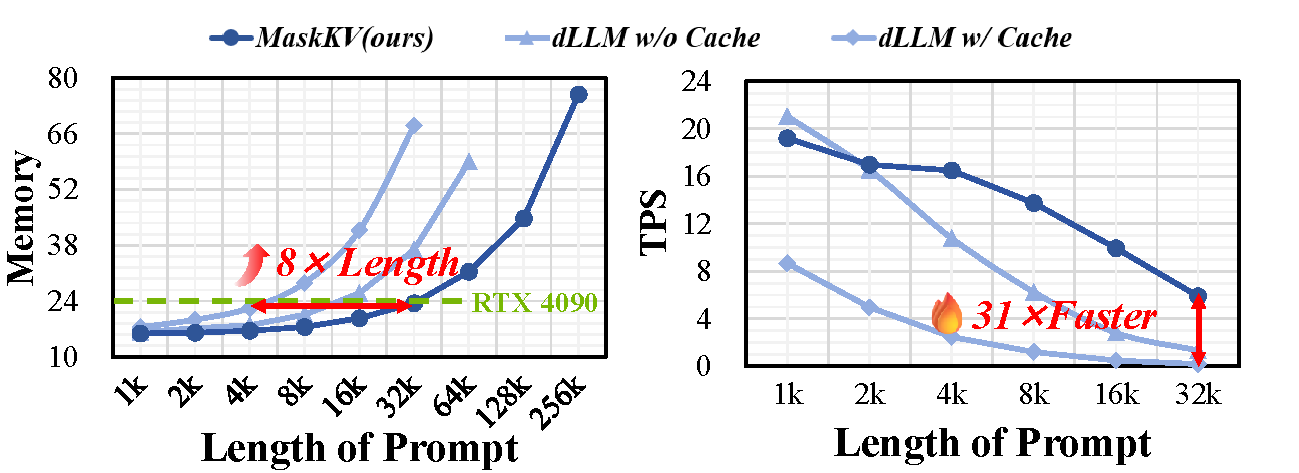
\includegraphics[width=\columnwidth]{figure/efficiency_new.pdf}
  \caption{Analysis on latency and memory reduction.}
  \label{fig:efficiency}
\end{figure}

\noindent \textbf{Efficiency in Speed and Memory.}
Our method markedly improves throughput and memory efficiency for long-context inference. 
We introduce two implementation optimizations, \textit{Prompt-State Exclusion} and \textit{Mask-Only Projection} (details in Appendix~\ref{sec:maskkv_details}). 
With these techniques, the memory footprint of \emph{MaskKV} becomes comparable to, or even lower than, that of LLaDA under identical configurations. 
At a 32K-token context, it achieves \textbf{31$\times$} faster decoding and \textbf{65\%} lower peak memory than LLaDA, supporting up to \textbf{8$\times$} longer prompts on an RTX 4090 GPU. 
Ablation results isolating the effects of cache eviction and the proposed optimizations are provided in Tab.~\ref{tab:ablation_memory}.

\subsection{Ablation Study} 
\noindent \textbf{Effect of Base Rates $\alpha$ and $\beta$.}
\begin{figure}[t]
  \centering
  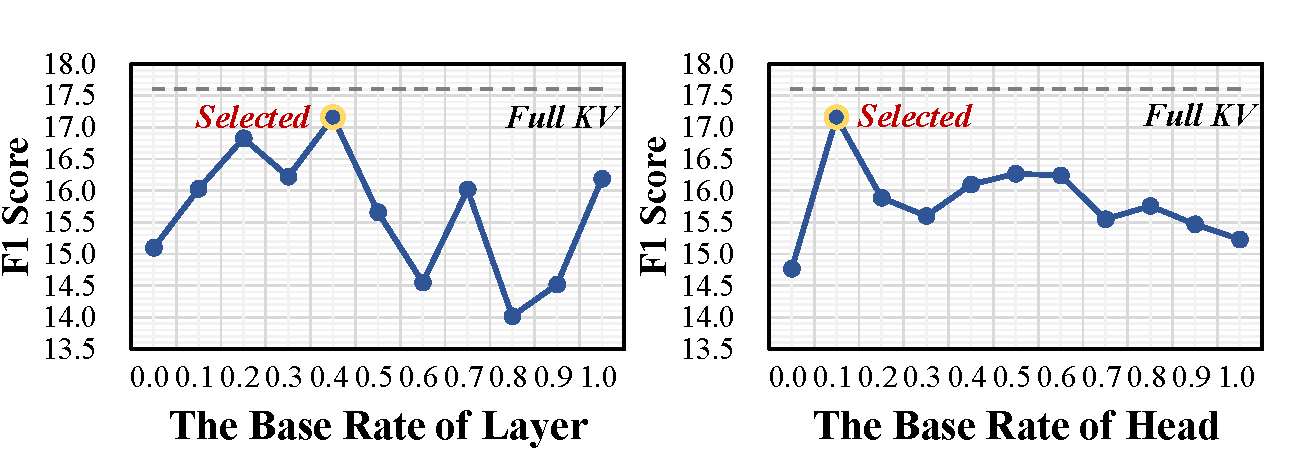
\includegraphics[width=\columnwidth]{figure/hy_new.pdf}
  \caption{Impact of base rate on model performance.}
  \label{fig:hy}
\end{figure}
The base rate of head ($\alpha$) and layer ($\beta$) represent uniform budget floors for attention heads and network layers, respectively.
These base rates first guarantee each unit a minimal share, after which the remaining budget is redistributed according to estimated importance.
Excessively large values drive allocations toward near‑uniformity, diluting capacity for critical modules, whereas overly small values make the policy too aggressive and unstable.
Empirical results (Fig.~\ref{fig:hy}) show that setting $\alpha=0.1$ 
and $\beta=0.4$ provides the most stable accuracy and key-value (KV) budgets, while 
still concentrating resources where they matter most.

\begin{table}[t]
\centering
\small
\renewcommand{\arraystretch}{1.15}
\setlength{\tabcolsep}{10pt}
\begin{tabular}{l l}
\toprule
\textbf{Variant} & \textbf{Performance (Avg) } \\
\midrule
Mask-Voting  & $35.39$ \\
\midrule
\multicolumn{2}{c}{\textit{Layer Budget Allocation}} \\
\midrule
+SqueezeAttention          & $35.62_{\textcolor{green}{\scriptsize +0.23}}$ \\
+PyramidKV          & $33.52_{\textcolor{black!50}{\scriptsize -1.87}}$ \\
\rowcolor{lightgreen}
+Boundary-Aware(online)  & $\mathbf{35.65}_{\textcolor{green}{\scriptsize +0.26}}$ \\
\rowcolor{lightgreen}
+Boundary-Aware(offline)  & $\mathbf{35.74}_{\textcolor{green}{\scriptsize +0.35}}$ \\
\midrule
\multicolumn{2}{c}{\textit{Head Budget Allocation}} \\
\midrule
+adaKV         & $35.70_{\textcolor{green}{\scriptsize +0.32}}$ \\
\rowcolor{lightgreen}
+Prompt-Preference    & $\mathbf{35.96}_{\textcolor{green}{\scriptsize +0.57}}$ \\
\midrule
\multicolumn{2}{c}{\textit{Layer + Head Allocation}} \\
\midrule
\rowcolor{lightgreen}
\textbf{MaskKV (Ours) } & $\mathbf{36.27}_{\textcolor{green}{\scriptsize +0.88}}$ \\
\bottomrule
\end{tabular}
\caption{Ablation study of budget allocation.}
\label{tab:ablation}
\end{table}


\noindent \textbf{Mask-Token Voting and Budget Allocation.}
Our Mask-Voting consistently achieves superior performance over other token selection methods by directly leveraging mask queries, which helps avoid local bias and better identify influential tokens. More comprehensive comparisons with alternative token selection strategies are provided in  Tab.~\ref{tab:voting}. In addition, our budget allocation strategies Boundary-Aware at the layer level and Prompt-Preference at the head level both outperform competing approaches in Tab.~\ref{tab:ablation}.

